%%%%%%%%%%%%%%%%%%%%%%%%%%%%%%%%%%%%%%%%%%%%%%%%%%%%%%%%%%%%%%%%%%%%%%%%%%%%%%%%
%2345678901234567890123456789012345678901234567890123456789012345678901234567890
%        1         2         3         4         5         6         7         8

\documentclass[letterpaper, 10 pt, conference]{ieeeconf}  % Comment this line out if you need a4paper

%\documentclass[a4paper, 10pt, conference]{ieeeconf}      % Use this line for a4 paper

\IEEEoverridecommandlockouts                              % This command is only needed if
                                                          % you want to use the \thanks command

\overrideIEEEmargins                                      % Needed to meet printer requirements.

% See the \addtolength command later in the file to balance the column lengths
% on the last page of the document

% The following packages can be found on http:\\www.ctan.org
%\usepackage{graphics} % for pdf, bitmapped graphics files
%\usepackage{epsfig} % for postscript graphics files
%\usepackage{mathptmx} % assumes new font selection scheme installed
%\usepackage{times} % assumes new font selection scheme installed
%\usepackage{amsmath} % assumes amsmath package installed
%\usepackage{amssymb}  % assumes amsmath package installed
\usepackage{cite}      % Written by Donald Arseneau
                        % V1.6 and later of IEEEtran pre-defines the format
                        % of the cite.sty package \cite{} output to follow
                        % that of IEEE. Loading the cite package will
                        % result in citation numbers being automatically
                        % sorted and properly "ranged". i.e.,
                        % [1], [9], [2], [7], [5], [6]
                        % (without using cite.sty)
                        % will become:
                        % [1], [2], [5]--[7], [9] (using cite.sty)
                        % cite.sty's \cite will automatically add leading
                        % space, if needed. Use cite.sty's noadjust option
                        % (cite.sty V3.8 and later) if you want to turn this
                        % off. cite.sty is already installed on most LaTeX
                        % systems. The latest version can be obtained at:
                        % http://www.ctan.org/tex-archive/macros/latex/contrib/supported/cite/

\usepackage[dvips]{graphicx}  % Written by David Carlisle and Sebastian Rahtz
                        % Required if you want graphics, photos, etc.
                        % graphicx.sty is already installed on most LaTeX
                        % systems. The latest version and documentation can
                        % be obtained at:
                        % http://www.ctan.org/tex-archive/macros/latex/required/graphics/
                        % Another good source of documentation is "Using
                        % Imported Graphics in LaTeX2e" by Keith Reckdahl
                        % which can be found as esplatex.ps and epslatex.pdf
                        % at: http://www.ctan.org/tex-archive/info/

%\usepackage{amsmath}   % From the American Mathematical Society
                        % A popular package that provides many helpful commands
                        % for dealing with mathematics. Note that the AMSmath
                        % package sets \interdisplaylinepenalty to 10000 thus
                        % preventing page breaks from occurring within multiline
                        % equations. Use:
\usepackage{multirow}
%\usepackage[left=0.71in,top=0.94in,right=0.71in,bottom=1.18in]{geometry}
%\setlength{\columnsep}{0.24in}
% correct bad hyphenation here
%\hyphenation{op-tical net-works semi-conduc-tor IEEEtran}
\usepackage{mathtools}   % loads »amsmath«
\usepackage{amssymb,amsmath}
\usepackage{amsfonts}
\usepackage{color}


\title{\LARGE \bf
Simultaneous Coordinate Calibrations by Solving the AX=YB Problem without Correspondence*
}


\author{Haiyuan Li$^{1}$, Qianli Ma$^{2}$, Tianmiao Wang$^{1}$ and Gregory Chirikjian$^{2}$% <-this % stops a space
\thanks{*This work is partially
supported by NSF Grant RI-Medium: \#IIS-1162095}% <-this % stops a space
\thanks{$^{1}$Haiyuan Li and Tianmiao Wang is with the School of Mechanical Engineering and Automation, Beihang University,
        ,Beijing 100191, China
        {\tt\small haiyuanli@hotmail.com}, {\tt\small itm@buaa.edu.cn}}%
\thanks{$^{2}$Qianli Ma and Gregory Chirikjian with the Department of Mechanical Engineering, Johns Hopkins University,
        Baltimore, MD 21218, USA
        {\tt\small mqianli1@jhu.edu}, {\tt\small gregc@jhu.edu}}%
}

\begin{document}



\maketitle
\thispagestyle{empty}
\pagestyle{empty}


%%%%%%%%%%%%%%%%%%%%%%%%%%%%%%%%%%%%%%%%%%%%%%%%%%%%%%%%%%%%%%%%%%%%%%%%%%%%%%%%
\begin{abstract}

In image-guided systems, the relative transformations of hand-eye ($X$) and robot-world ($Y$) coordinates have to be calculated and a simultaneous solution is useful in sensor calibration problem. Due to the asynchrony of sensors' timing, the exact correspondence between $A$ and $B$ is unknown, and a common scenario is when there is a constant shift between the two data streams. A probabilistic method is presented to solve the
homogeneous matrix equations without a priori knowledge of the correspondence. Using the Euclidean-Group invariants, an exact solution can be found. For noisy and shifted data streams, we numerically simulated the proposed method, and the results show the efficiency and robustness.

\end{abstract}


%%%%%%%%%%%%%%%%%%%%%%%%%%%%%%%%%%%%%%%%%%%%%%%%%%%%%%%%%%%%%%%%%%%%%%%%%%%%%%%%

\section{Introduction}
% no \PARstart

Image-guided system has been widely used in robotics such as robot assisted surgery, automatic guided vehicle, etc. Sensors such as a camera, a laser scanner or an ultrasound probe are usually mounted on the distal end of a robotic manipulator. For a typical ``hand-eye'' system as described above, the relative transformation of the sensor with respect to the end-effector should be accurately calibrated, and it is often characterized as the well known $\textbf{AX=XB}$ problem. A variation of this problem is the $\textbf{AX=YB}$ problem, where both the hand-eye transformation and the pose of the robot base with respect to the world frame need to be calibrated. In a typical environment setup, the relationships among the sensor frame, robot frame and world frame are variant and the uncertainties exist. Therefore, simultaneous coordinate calibrations have to be determined frequently in order to enable the robots to respond to dynamic environments.

In the $\textbf{AX=YB}$ problem, $As$ and $Bs$ can be respectively obtained via different sensors. The data streams can be in an asynchronous fashion due to the different working frequencies of the sensors. The asynchrony causes a shift between the two streams of data which damages the correspondence between $As$ and $Bs$. In this paper, a novel method is presented to solve for $X$ and $Y$ without the need to know a priori knowledge of the correspondence between $As$ and $Bs$.

\begin{center}
\begin{figure}[htbp]
\centering
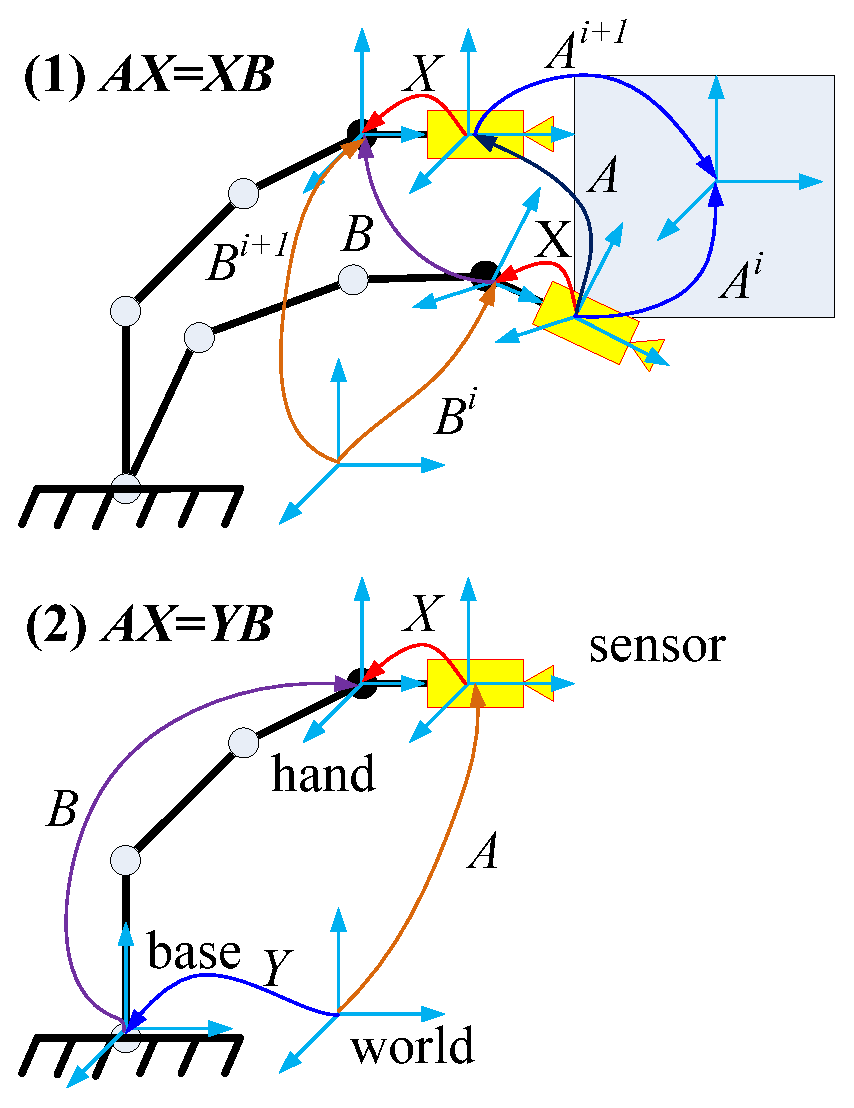
\includegraphics[width=3.2in]{fig1.eps}
\caption{
(1) The hand-eye and robot-world calibration problem which is formulated as AX=YB (The universal robot as shown in the picture is owned by professor Emad Boctor in the Johns Hopkins University). (2) The hand-eye calibration problem which is formulated as AX=XB.
}
\label{fig1}
\end{figure}
\end{center}
The hand-eye calibration problem can be modeled as $\textbf{AX = XB}$, where $A$ and $B$ are the homogeneous transformation matrices describing  the relative motions of the end-effector and the  sensor respectively. As shown in Fig.~\ref{fig1}, $A = A^{i}(A^{i+1})^{-1}$ and  $B = B^{i}(B^{i+1})^{-1}$. Given multiple pairs of $(A_i,B_i)$ with correspondence, many methods have been proposed to solve for $X$. To the best of the authors' knowledge, Shiu \cite{Shiu1989} and Tsai \cite{Tsai1989} are the first to solve the $AX = XB$ sensor calibration problem. The other methods include but are not limited to the quaternion, dual quaternion, screw theory, Lie group theory, convex optimization and gradient descent methods \cite{Wang1992,Park1994,Horaud1995,Daniilidis1999,Fassi2005,Zhao2011,Ackerman2014a}. All of the methods above assume a prior knowledge of exact correspondence between $A_i$ and $B_i$. For data streams $\{A_i\}$ and $\{B_j\}$ that are asynchronous, several methods have been proposed in the literature to solve for $X$ using data without correspondence.  Theses methods assume that there is exact knowledge of the correspondence between $\{A\}$ and $\{B\}$ \cite{Ackerman2013a,Ackerman2013,Ackerman2014}.

Simultaneous estimation of the hand-eye and robot-world transformations has been viewed as the $\textbf{AX=YB}$ problem. As shown in Fig.~\ref{fig1}, $Y$ is the transformation from the robot base to the world frame, $A$ denotes the pose of the sensor in the world frame and $B$ is the transformation from the the end-effector to its fixed base. The $A$ and $B$ in $\textbf{AX=YB}$ are different from those in $\textbf{AX=XB}$ where the former uses absolute transformations and the latter uses relative transformations. This problem has been solved by many different methods such as the Kronecker product, quaternion, dual quaternion, and nonlinear optimization methods \cite{Zhuang1994,dornaika1998simultaneous,Hirsh2001, ernst2012non,strobl2006optimal,Li2010,Shah2013,Heller2014}. Simulatneous calibrations of $X$ and $Y$ can be problematic in that all the methods above assume exact correspondence between $\{A_i\}$ and $\{B_j\}$, which is not the case in the real world. Another similar problem involves the calibration of multiple robots in terms of hand-eye, tool-flange and robot-robot system, and it is formulated as the $\textbf{AXB=YCZ}$ problem \cite{Wang2014}. Simultaneous solution for $X$ and $Y$ in $\textbf{AX=YB}$ problem is a challenging issue. In the above methods, the correspondence between $A$ and $B$ is known a prior. In this paper, we focus on a case of $\textbf{AX=YB}$ problem where there is  no a priori knowledge of the correspondence between the data streams.

The rest of the paper is organized as follows. In Section
\ref{sect2}, a novel probabilistic method is presented to solve for $X$ and $Y$. In Section \ref{sect3}, an algorithm involving both correlation theorem and Euclidean group invariants is proposed to recover the correspondence between $\{A_i\}$ and $\{B_j\}$. The simulation results which deal with noisy data without correspondence are illustrated in Section \ref{sect4}. Finally, conclusions are drawn based on the numerical results and possible future works are pointed out.

\section{Solving AX=YB using a probabilistic method on motion groups}
\label{sect2}
In this section, a brief introduction to the concepts of probability density function on the special Eucledian group $SE(3)$ is presented and the probabilistic representation of $AX=YB$ are derived.

Any rigid transformation matrix can be viewed as a group element of $SE(3)$ :
\begin{equation}\label{equ0}
    H(R,t)=\left(
             \begin{array}{cc}
               R & t \\
               0^{T} & 1 \\
             \end{array}
           \right) \in SE(3), \; \; R \in SO(3)
\end{equation}
where $SO(3)$ denotes the special orthogonal group, $t \in \mathbb{R}^3 $ is translational vector and $H$ is symbol for group element.

Given a large set of pairs $(A_{i},B_{i})\in SE(3)\times SE(3)$ where $i=1,\cdots,n$, the following equation is true if the correspondence is known as a priori:

\begin{equation}\label{equ1}
A_{i}X=YB_{i}.
\end{equation}
For a group element $H \in SE(3)$, a Dirac delta function $\delta(H)$ is defined to be finite only at the identity and zero elsewhere:

\begin{equation}\label{equ2}
\delta{(H)}=
\left\{
\begin{array}{ll}
+\infty, & H=I \\
0, & H \neq I
\end{array}
\right.
\end{equation}
It also satisfies the identity constraint as:

\begin{equation}\label{equ3}
\int_{SE(3)}\delta{(H)}dH=1.
\end{equation}

A shifted Dirac delta function can be defined as $\delta_{A}(H)=\delta{(A^{-1}H)}$. Given $K,H \in SE(3)$ and two well-defined functions $f_{1}, f_{2} \in \left(L^1 \cap L^2 \right)(SE(3))$, their convolution on $SE(3)$ is defined as:

\begin{equation}\label{equ4}
(f_{1}\ast f_{2})(H)=\int_{SE(3)}f_{1}(K)f_{2}(K^{-1}\circ H)dK.
\end{equation}
Employing the properties of $\delta$ function, it is straightforward to see that:

\begin{equation}\label{equ5}
(f\ast \delta)(H)=\int_{SE(3)}f(K)\delta(K^{-1}\circ H)dK=f(H).
\end{equation}
Therefore, for each $A_{i}$ and $B_{i}$, the following equations can be obtained:

\begin{IEEEeqnarray}{l}\label{equ6}
(\delta_{A_{i}}\ast \delta_{X})(H)=\delta(A_{i}^{-1} H X^{-1}) \IEEEyessubnumber
\\*
(\delta_{Y}\ast \delta_{B_{i}})(H)=\delta(Y^{-1} H B_{i}^{-1}). \IEEEyessubnumber
\end{IEEEeqnarray}
Using Eq.($\ref{equ1}$), the above two equations can be combined into a single equation as:

\begin{equation}\label{equ7}
(\delta_{A_{i}}\ast \delta_{X})(H)=(\delta_{Y}\ast \delta_{B_{i}})(H)
\end{equation}

Define the probability density function of $\{A_i\}$ and $\{B_i\}$ as:
\begin{IEEEeqnarray}{l}\label{equ8}
f_{A}(H)=\frac{1}{n}\sum_{i=1}^{n} \delta_{A_{i}}(H) \IEEEyessubnumber
\\*
f_{B}(H)=\frac{1}{n}\sum_{i=1}^{n} \delta_{B_{i}}(H) \IEEEyessubnumber
\end{IEEEeqnarray}
Using the distributivity of convolution, add $n$ instances of Eq.(\ref{equ8}) and substitute Eq.(\ref{equ7}) in can give:
\begin{equation}\label{equ9}
(f_{A_{i}}\ast \delta_{X})(g)=(\delta_{Y}\ast f_{B_{i}})(g)
\end{equation}

% small relative motions are calculated using consecutive transformations. Take $\{A_i\}$ for example, one metric % of the distance between $A_i$ and $A_{i+1}$ can be defined as:

% \begin{eqnarray}\label{equ10}
% d^{2}(A_{i},A_{i+1})=\parallel \Delta A \parallel_{W}^{2} = trace[(\Delta A)W(\Delta % A)^{T}] = \epsilon,\nonumber \\
% \end{eqnarray}
% where $\Delta A = A_{i}-A_{i+1}$ and $0 < \epsilon \ll 1 $.

Each of the data stream $\{A_i\}$ and $\{B_i\}$ is generated using Gaussian distribution over $SE(3)$. The convolution of two "highly focused" probability density functions (PDF) have some interesting properties that can be used to solve for $X$. In particular, define the mean $M$ and covariance $\Sigma$ of a probability density function on $SE(3)$ as:

\begin{IEEEeqnarray}{l}\label{equ11}
\int_{SE(3)}log(M^{-1}H))f(H)dH=0 \IEEEyessubnumber
\\*
\Sigma = \int_{SE(3)}log^{\vee}(M^{-1}H)[log^{\vee}(M^{-1}H)]^{T}f(H)dH. \IEEEyessubnumber
\end{IEEEeqnarray}
Then the corresponding discrete version is:

\begin{IEEEeqnarray}{l}\label{equ12}
\sum_{i=1}^{n}log(M^{-1}H))=0 \IEEEyessubnumber
\\*
\Sigma = \sum_{i=1}^{n}log^{\vee}(M^{-1}H)[log^{\vee}(M^{-1}H)]^{T}. \IEEEyessubnumber
\end{IEEEeqnarray}

Given $\{A_i\}$ where the cloud of frames ${A_{i}}$ clustering around $M_{A}$, an iterative formula can be used for computing $M_{A}$ \cite{Wang2008} as:

\begin{equation}\label{equ13}
    ^{k+1}M_{A} = ^{k}M_{A} \circ exp[\frac{1}{n}\sum_{i=1}^{n}log(^{k}M_{A}^{-1}\circ A_{i})]
\end{equation}

An initial estimate of the iterative procedure can be chosen as $^{0}M_{A}=\frac{1}{n}\sum_{i=1}^{n}log(A_{i})$, then a local minimum of $M_A$ is obtained by solving a nonlinear optimization problem with the cost function being $|| \sum_{i=1}^{n}log(M_{A}^{-1}A_{i}) ||^{2}$. A similar procedure can be used to compute $M_B$. $\Sigma_A$ and $\Sigma_B$ are then straight forward to compute given known $M_A$ and $M_B$.

The mean and covariance for the convolution $(f_{1} \ast f_{2})(g)$ of two highly focused functions $f_{1}$ and $f_{2}$ are calculated as in \cite{Wang2008}:

\begin{IEEEeqnarray}{l}\label{equ14}
M_{1 \ast 2} = M_{1}M_{2} \IEEEyessubnumber
\\*
\Sigma_{1 \ast 2} = Ad(M_{2}^{-1})\Sigma_{1}Ad^{T}(M_{2}^{-1}) + \Sigma_{2}. \IEEEyessubnumber
\end{IEEEeqnarray}
where

$$Ad(H)=\left(
               \begin{array}{cc}
                 R & O \\
                 \hat{t}R & R \\
               \end{array}
             \right).$$

Because $X$ and $Y$ are constant, their corresponding PDF will be $\delta_{X}(g)$ and $\delta_{Y}(g)$, of which the mean and covariance are $M_{X} = X$, $\Sigma_{X} = \mathbb{O}_{6 \times 6}$ and $M_{Y} = Y$, $\Sigma_{Y} = \mathbb{O}_{6 \times 6}$, respectively. Therefore, the following equations can be obtained using Eq.(\ref{equ14}):

\begin{IEEEeqnarray}{l}
M_{A} X = Y M_{B} \IEEEyessubnumber\label{equ15a}
\\*
Ad(X^{-1})\Sigma_{A}Ad^{T}(X^{-1}) = \Sigma_{B}. \IEEEyessubnumber\label{equ15b}
\end{IEEEeqnarray}

To solve the above equations, Eq.(\ref{equ15a}) is decomposed into a rotational equation and a translational equation as below:

\begin{IEEEeqnarray}{l}
R_{M_{A}} R_{X} = R_{Y} R_{M_{B}} \IEEEyessubnumber\label{equ16a}
\\*
R_{M_{A}} t_{X} + t_{M_{A}}= R_{Y} t_{M_{B}} + t_{Y}. \IEEEyessubnumber\label{equ16b}
\end{IEEEeqnarray}
$\Sigma_{A}$ and $\Sigma_{B}$ can be decomposed into blocks as
$\left(\begin{array}{cc}
       \Sigma_{A}^{1} & \Sigma_{A}^{2} \\
       \Sigma_{A}^{3} & \Sigma_{A}^{4} \\
       \end{array}
       \right)$
and
$\left(\begin{array}{cc}
       \Sigma_{B}^{1} & \Sigma_{B}^{2} \\
       \Sigma_{B}^{3} & \Sigma_{B}^{4} \\
       \end{array}
       \right)$, respectively. Knowing that
$ X^{-1} = \left(\begin{array}{cc}
       R_{X}^{T} & -R_{X}^{T}t_{X}  \\
       0 & 1 \\
       \end{array}
       \right)$,
then the first two blocks of Eq.(\ref{equ15b}) can be written as follows:

\begin{IEEEeqnarray}{l}
\Sigma_{M_{B}}^{1} = R_{X}^{T}\Sigma_{M_{A}}^{1} R_{X} \IEEEyessubnumber\label{equ17a}
\\*
\Sigma_{M_{B}}^{2} = R_{X}^{T}\Sigma_{M_{A}}^{1} R_{X} (\widehat{R_{X}^{T}t_{X}}) + R_{X}^{T}\Sigma_{M_{A}}^{2}R_{X}.
 \IEEEyessubnumber\label{equ17b}
\end{IEEEeqnarray}
Because Eq.(\ref{equ17a}) is a similarity transformation between $\Sigma_{M_{B}}^{1}$ and $\Sigma_{M_{A}}^{1}$, they share the same eigenvalues and can be eigendecomposed into   $\Sigma_{M_{A}}^{1}=Q_{M_{A}}\Lambda Q_{M_{A}}^{T}$ and $\Sigma_{M_{B}}^{1}=Q_{M_{B}}\Lambda Q_{M_{B}}^{T}$ where $\Lambda$ is a diagonal matrix whose diagonal elements are the eigenvalues of $\Sigma_{M_{A}}^{1}$ (or $\Sigma_{M_{B}}^{1}$), and $Q_{M_{A}}$ (or $Q_{M_{B}}$) is a square matrix whose columns are the corresponding eigenvectors. The following equation is obtained after substituting $\Sigma_{M_{B}}^{1}$ and $\Sigma_{M_{A}}^{1}$ into Eq.(\ref{equ17a}):

\begin{equation}\label{equ18}
    \Lambda = (Q_{M_{A}}^{T}R_{X}^{T}Q_{M_{B}}) \Lambda (Q_{M_{B}}^{T}R_{X}Q_{M_{A}})= P \Lambda P^{T}
\end{equation}
where $P=Q_{M_{A}}^{T}R_{X}Q_{M_{B}}$. If $Q_{M_{A}}$ and $Q_{M_{B}}$ are further constrained to be rotation matrices, then a rotation matrix $P$ that satisfies Eq.(\ref{equ18}) can be one of $\mathcal{P}$ or $\mathcal{-P}$ :

\begin{equation}\label{equ19}
\begin{split}
{\cal P} = \left\{ \left(\begin{array}{ccc}
1\,\, & 0 \,\, & 0 \,\, \\
0 & 1 & 0\\
0 & 0 & 1 \end{array}\right) , \left(\begin{array}{ccc}
-1 & 0 & 0 \\
0 & -1 & 0\\
0 & 0 & 1 \end{array}\right), \right.\\
\left. \left(\begin{array}{ccc}
-1 & 0 & 0 \\
0 & 1 & 0\\
0 & 0 & -1 \end{array}\right), \left(\begin{array}{ccc}
1 & 0 & 0 \\
0 & -1 & 0\\
0 & 0 & -1 \end{array}\right)\right\}.
\end{split}
\end{equation}

Therefore, there are eight candidates of $R_{X}$ which can be calculated via $R_{X}=Q_{M_{A}}PQ_{M_{B}}^T$, and the corresponding $t_{X}$ can be obtained  from Eq.(\ref{equ17b}). Given known $X$, $Y$ can be solved for by $Y = M_A^{-1}XM_B^{-1}$. At last, eight candidate pairs of  $\{X_{k},Y_{k}\}$ can be obtained as:

\begin{equation}\label{equ20}
\begin{array}{cc}
X_{k}= \left( \begin{array}{cc}
       R_{X_k} & t_{X_k} \\
       \mathbf{0}^{T} & \mathbf{1}\\
\end{array} \right),&
Y_{k}= \left( \begin{array}{cc}
       R_{Y_k} & t_{Y_k} \\
       \mathbf{0}^{T} & \mathbf{1}\\
\end{array} \right)
\end{array}
\end{equation}
where $k = 1,2,...,8$.

The problem then becomes selecting the best pair of $\{X_k, Y_k\}$ from the eight candidates.
Based on the screw theory, it is known that a homogeneous transformation $H$ can be expressed by the four screw parameters $(\theta,d,\mathbf{n},\mathbf{p})$ that define the $Pl\ddot{u}cker$ coordinates of the screw motion as:

\begin{equation}\label{equ21}
H = \left( \begin{array}{cc}
       e^{\theta \hat{\mathbf{n}}} & (\mathbf{I}_{3} - e^{\theta \hat{\mathbf{n}}})\mathbf{p} + d\mathbf{n} \\
       \mathbf{0}^{T} & \mathbf{1}
\end{array} \right)
\end{equation}
where $\theta$ is the angle of rotation, $d$ is the translation along the rotation axis, $\mathbf{n}$ is the unit vector representing the axis of rotation and $\mathbf{p}$ is the position of the line to the origin with $\mathbf{p} \cdot \mathbf{n} = 0$.

Moreover, $A X_k = Y_k B$ can be written as $AX_k=X_k(X_k^{-1}Y_kB)$. Define $B^k = X_k^{-1}Y_kB$, and we will have $AX_k=X_kB^k$. There exist two Euclidean-Group invariant relationships for each pair of $(A_{i},B_{i}^k)( i = 1,\cdots,n; k=1,\dots,8)$ as follows:

\begin{equation}\label{equ22}
    \theta_{A_{i}}=\theta_{B_{i}^{k}}, d_{A_{i}}=d_{B_{i}^{k}}
\end{equation}

Among the eight pairs $(X_{k},Y_{k})$, one can find an optimal solution which  minimizes the cost function defined as:

\begin{equation}\label{equ23}
    (X,Y) = \mathop{\mathbf{arg}min}_{(X_{k},Y_{k})}\frac{1}{n} \sum_{i=1}^{n} (\parallel \theta_{A_{i}}-\theta_{B_{i}^{k}} \parallel + \parallel d_{A_{i}}-d_{B_{i}^{k}} \parallel)
\end{equation}
The correspondences between $\{A_i\}$ and $\{B_j\}$ need to be recovered to pick the optimal $X$ and $Y$.
\section{Solution with unknown correspondence between $A_{i}$ and $B_{i}^{k}$}
\label{sect3}

In most cases, the homogeneous transformations  $\{A_i\}$ and $\{B_j\}$ are calculated based on the data obtained from different sensors. Due to the asynchronous timing of the sensor readings, the correspondence between $\{A_{i}\}$ and $\{B_{j}^{k}\}$ is usually unknown. This section deals with the case where there is a shift between $\{A_i\}$ and $\{B_j\}$, and the Euclidean-Group invariants are used to recover the correspondence between the data streams. The advantage of the above probabilistic solution lies in that $X$ and $Y$ can be calculated even if there is not a priori knowledge of the correspondence. However, there are still eight possible candidates of $(X_{k},Y_{k})$ to choose from and by using Euclidean-Group invariants, it is straightforward to determine which pair is the optimal one if the correspondence between $A_{i}$ and $B_{i}^{k}$ can be known.

The Discrete Fourier Transform (DFT) decomposes a time-domain signal into its constituent frequencies. The input is a finite list of equally spaced samples of a function. Given a discrete signal consisting of a sequence of $N$ complex numbers $x_{0},x_{1},\cdots,x_{N-1}$, the DFT is denoted by $X_{\kappa} = \mathcal{F}({x_{n}})$ as:

\begin{equation}\label{equ24}
    X_{\kappa} = \sum_{n=0}^{N-1}x_{n}\cdot exp(-i\frac{2\pi}{N}n\kappa).
\end{equation}
where $i$ here is the imaginary unit.

The Inverse Discrete Fourier transform (IDFT) is denoted as:

\begin{equation}\label{equ25}
    x_{n} = \frac{1}{N}\sum_{n=0}^{N-1}X_{\kappa}\cdot exp(i\frac{2\pi}{N}n\kappa).
\end{equation}

The discrete convolution of two sequences $f_{n}$ and $g_{n}$  are defined

\begin{equation}\label{equ26}
    (f \ast g)(\tau)=\sum_{i=0}^{N}f(t_{i})g(t_{i}-\tau).
\end{equation}

In the convolution theorem, the Fourier transform of a convolution is the product of the Fourier transforms, namely:

\begin{equation}\label{equ27}
    f \ast g = \mathcal{F}^{-1} [\mathcal{F}(f) \cdot \mathcal{F}(g)].
\end{equation}

The correlation theorem indicates that the correlation function, $Corr(f,g)$, will be larger for a shift vector where the two sequences $f_n$ and $g_n$ can share more similar features. The correlation can be obtained based on the convolution theorem. The DFT of $Corr(f,g)$ is equal to the product of the DFT of $f_{n}$ and the complex conjugate $\mathcal{F}^{*}$ of the DFT of $g_n$:

\begin{equation}\label{equ28}
    Corr(f,g)=f \star g = \mathcal{F}^{-1}[\mathcal{F}(f) \cdot (\mathcal{F}(g))^{*}].
\end{equation}

Compared to the standard time-domain convolution algorithm, the complexity of the convolution by multiplication in the frequency domain is significantly reduced with the help of the convolution theorem and the fast Fourier transform (FFT).

Given two sequences $\{\theta_{A_{i}}\}$ and $\{\theta_{B_{i}^{k}}\}$ corresponding to  $\{A_{i}\}$ and $\{B_{i}^{k}\}$, the shift that is needed to recover the data correspondence is obtained as below.
Firstly, $\theta_{Ai}$ and $\theta_{B_{i}^{k}}$ are normalized as:

\begin{equation}\label{equ29}
    \theta_{1}=\frac{(\theta_{A_{i}}-\mu_{A_{i}})}{\sigma_{A_{i}}}, \theta_{2}=\frac{(\theta_{B_{i}^{k}}-\mu_{B_{i}^{k}})}{\sigma_{B_{i}^{k}}}
\end{equation}
where $\mu_{A_{i}}(\mu_{B_{i}^{k}})$ is the mean of $\theta_{A_{i}}(\theta_{B_{i}^{k}})$ and $\sigma_{A_{i}}(\sigma_{B_{i}^{k}})$ is the standard deviation.

Here, the correlation function $Corr(\theta_{1},\theta_{2})$  is the function of the time sequence index $n$ which describes the probability of these two sequences being separated by this particular unit. The index corresponding to the maximum of $Corr(\theta_{1},\theta_{2})$  indicates the amount of shift $\tau_{shift}$ between $\{\theta_{A_{i}}\}$ and $\{\theta_{B_{i}^{k}}\}$.

\begin{equation}\label{equ30}
    \tau_{shift} = \mathop{\mathbf{arg}max}_{index}(Corr(\theta_{1},\theta_{2}))
\end{equation}

Therefore, the correspondence between the two sequences can be found. The data of ${\theta_{A_{i}}}$ or ${d_{A_{i}}}$ are shifted by $-\tau_{shift}$ to obtain a sequence of new pairs $({\theta_{A_{i}}(i+\tau_{shift})},{\theta_{B_{i}^{k}}})$ and $({d_{A_{i}}(i+\tau_{shift})},{d_{B_{i}^{k}}})$, $max(0,\tau_{shift})\leq i \leq min(n,n+\tau_{shift})$. The data stream can be shifted back to regain correspondence to synchronize the data streams once the shift is computed, and the correct solution of $X$ and $Y$ can also be recovered by minimizing the cost function Eq.(\ref{equ23}) using the Euclidean-Group invariants as shown in Section \ref{sect2}.


\section{Simulation Studies}
\label{sect4}

\begin{center}
\begin{figure}
\centering
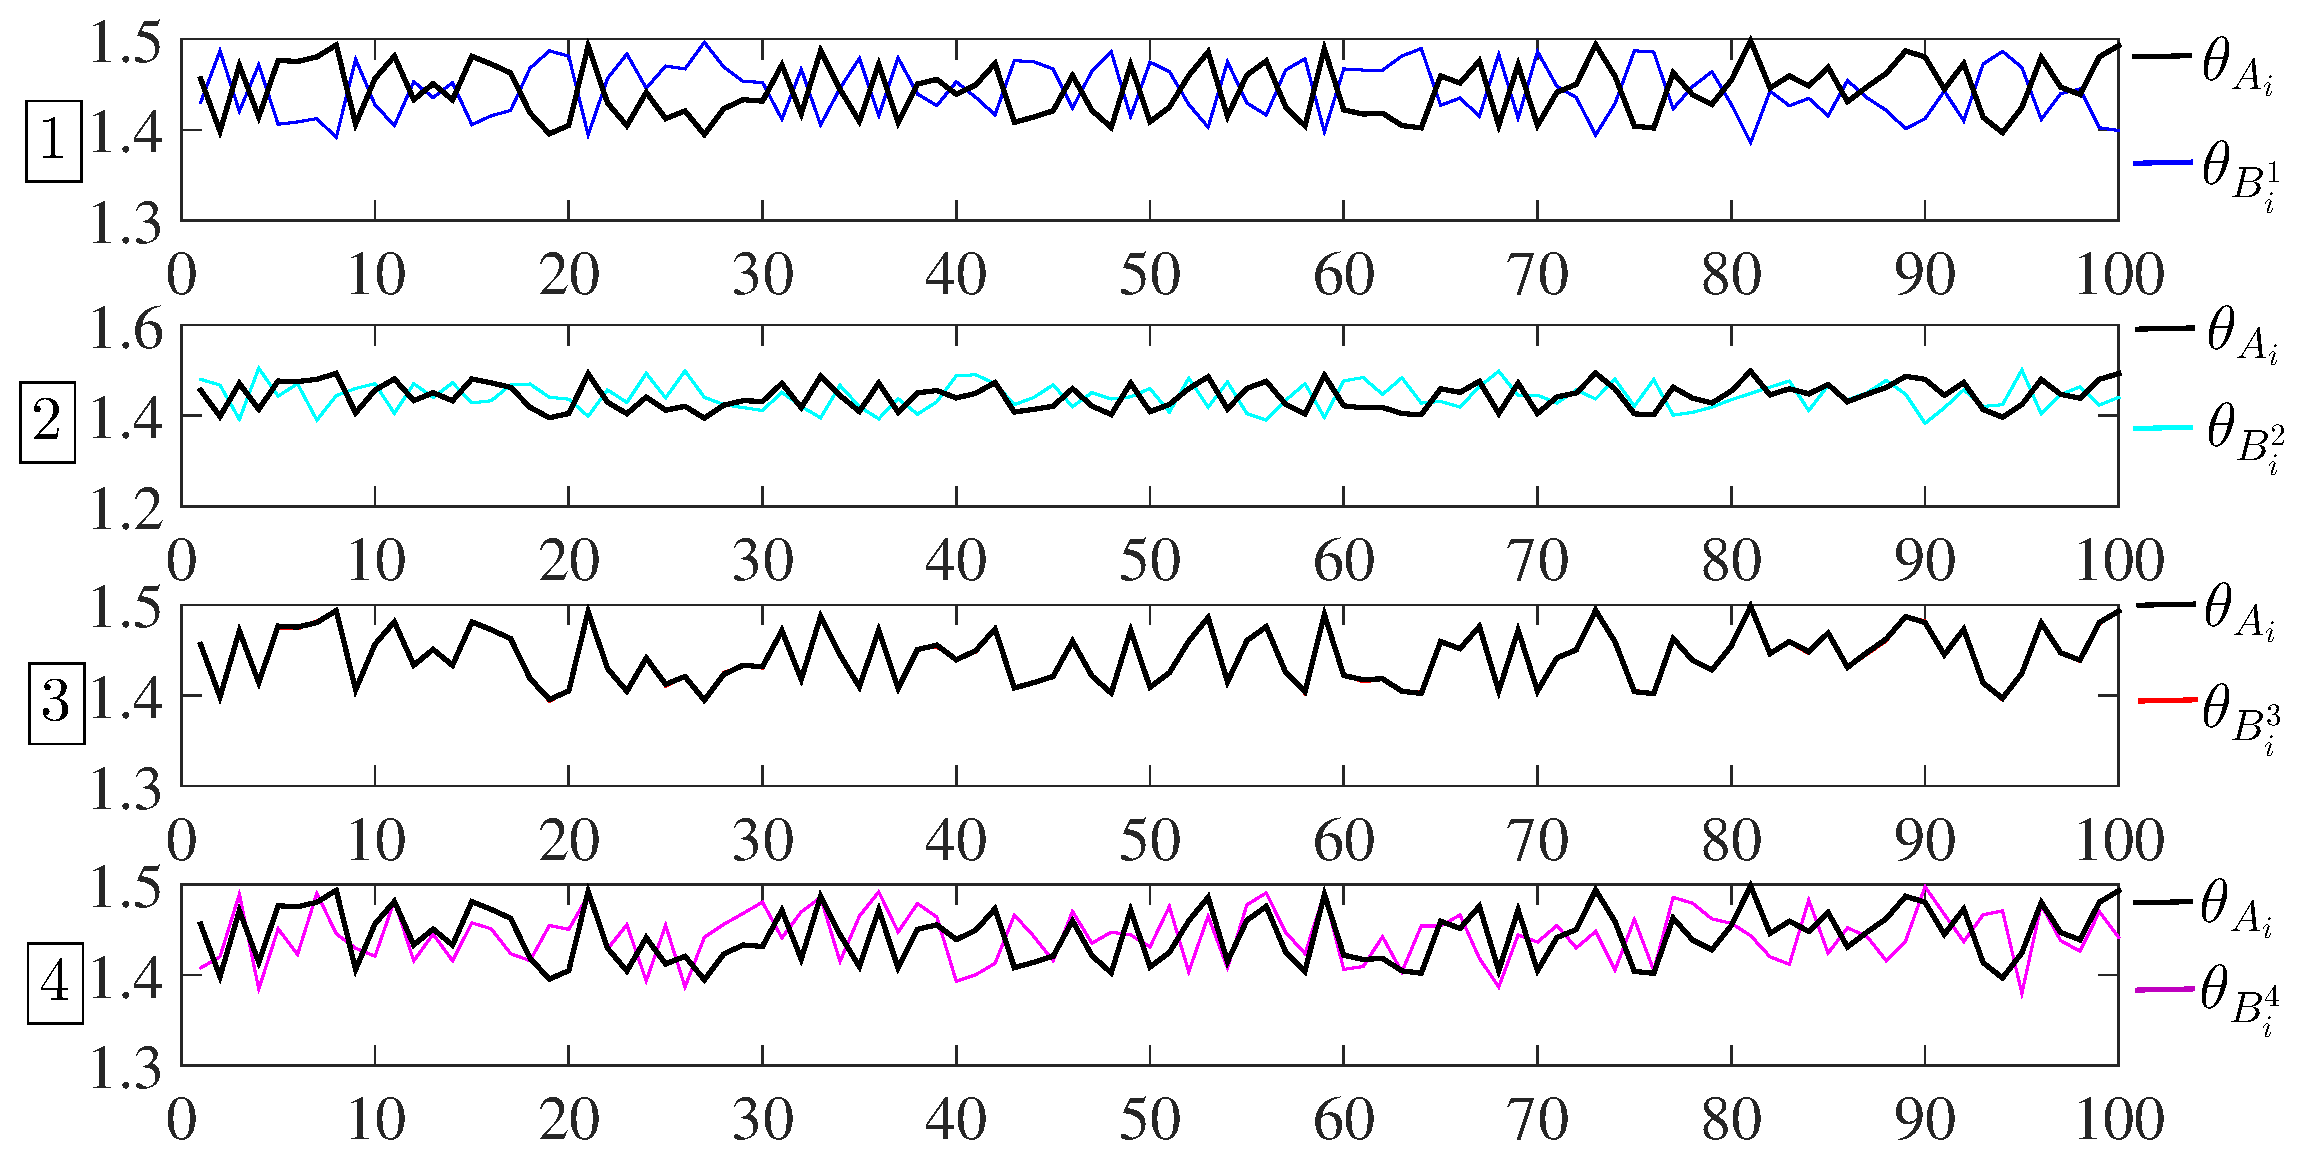
\includegraphics[width=3in]{fig2.eps}
\caption{
The errors of translation and rotations versus the shift between data streams $A$ and $B$
}
\label{fig2}
\end{figure}
\end{center}

\begin{figure}
\centering
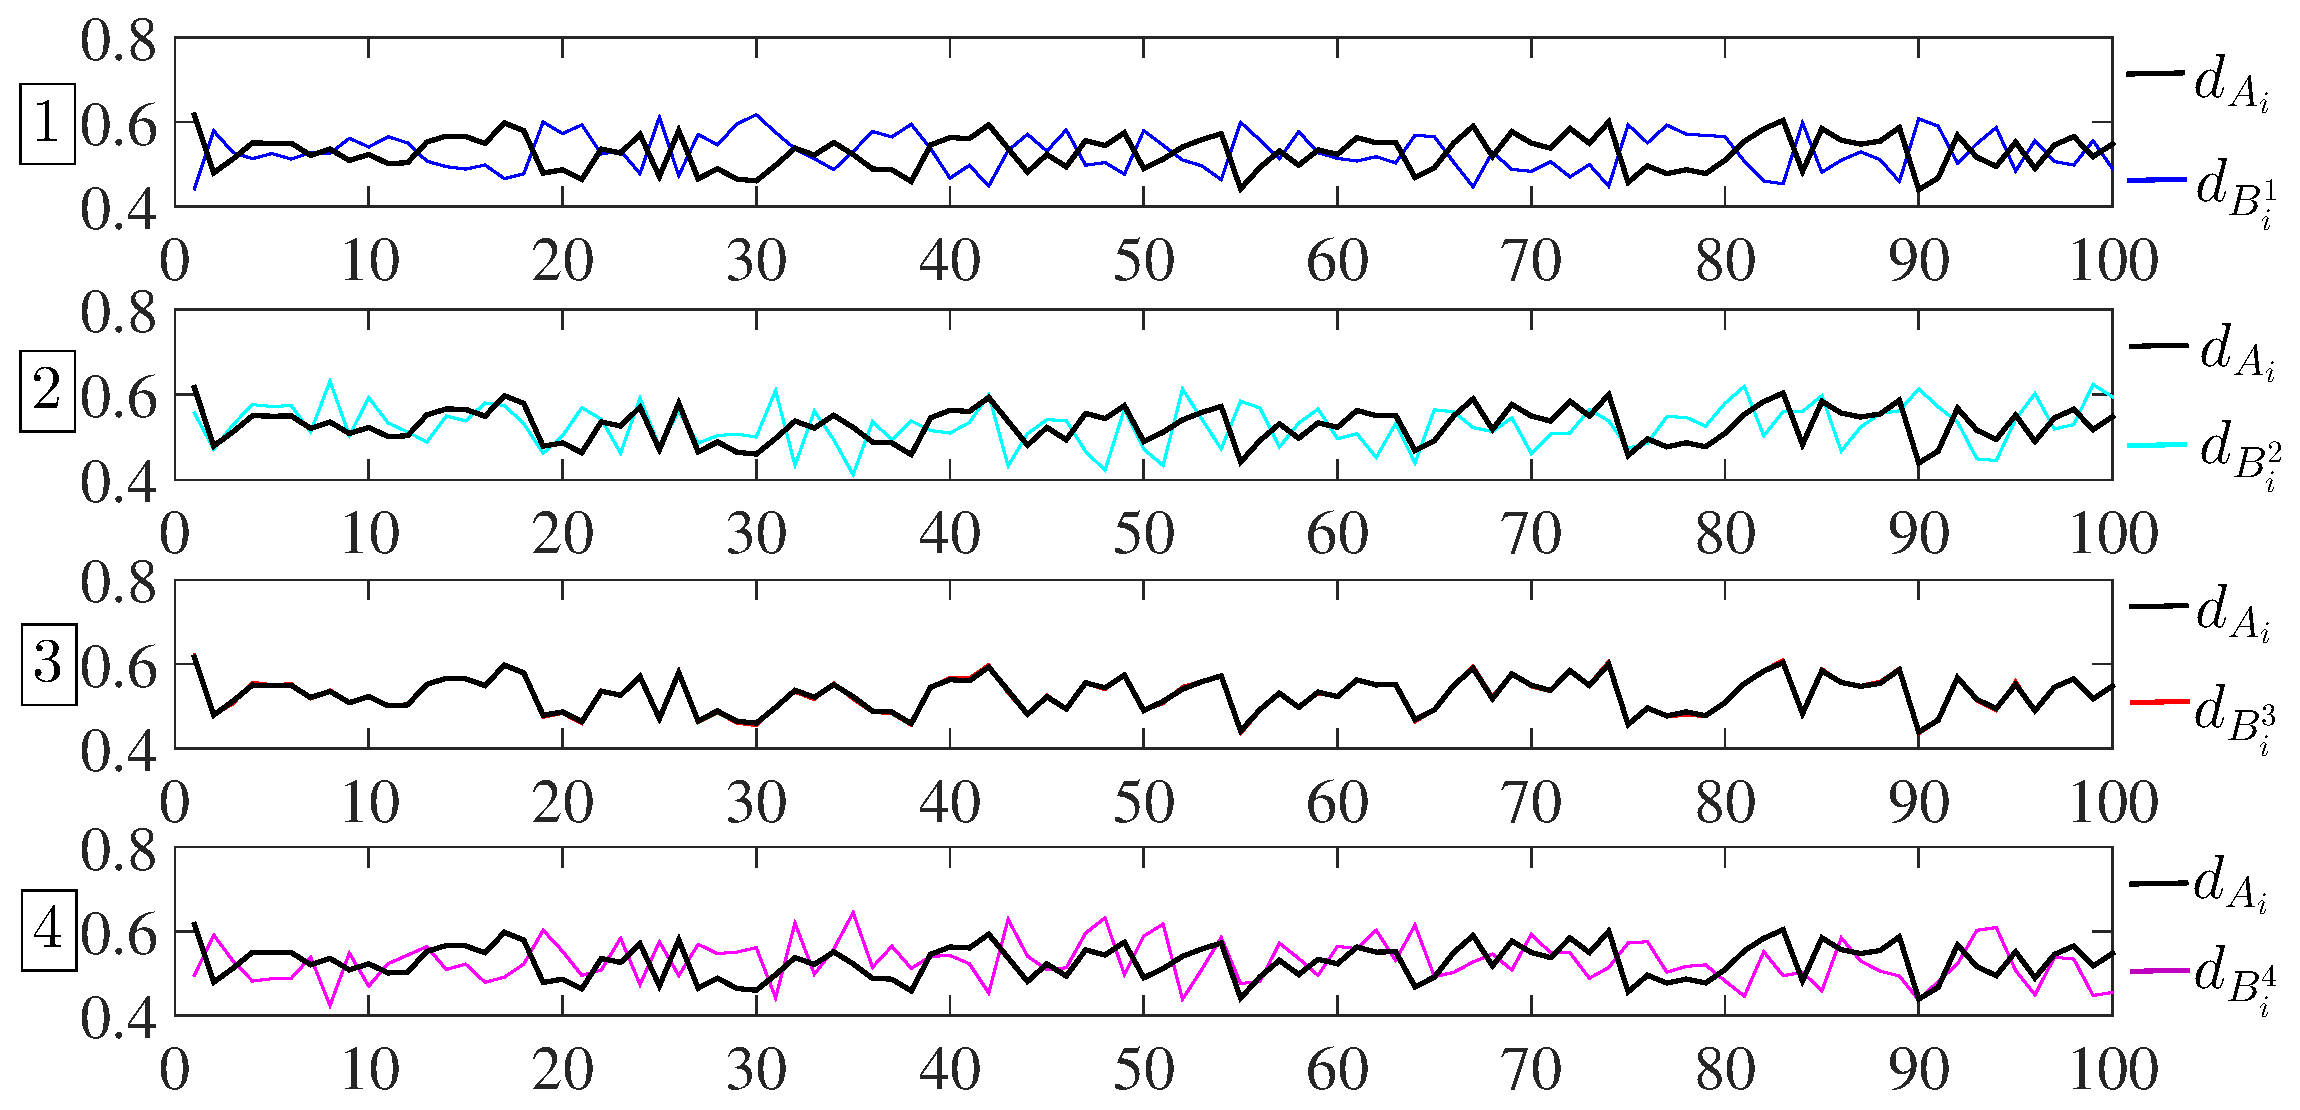
\includegraphics[width=3.2in]{fig3.eps}
\caption{
Box-and-Whisker plots  of translation and rotation erros versus noise covariance exerted to the data $B$.\vspace{6pt}
}
\label{fig3}
\end{figure}


For the numerical experiments in this section, the rotational and translational errors for $X$ and $Y$ are measured as  $Error(R_X) = \parallel log^{\vee} (R_{X_{Solved}}^{T}R_{X_{true}})\parallel$, $Error(t_X) = \parallel t_{X_{Solved}}-t_{X_{true}} \parallel$, $Error(R_Y) = \parallel log^{\vee} (R_{Y_{Solved}}^{T}R_{Y_{true}})\parallel$ and $Error(t_Y) = \parallel t_{Y_{Solved}}-t_{Y_{true}} \parallel$ respectively.

\begin{center}
\begin{figure}
\centering
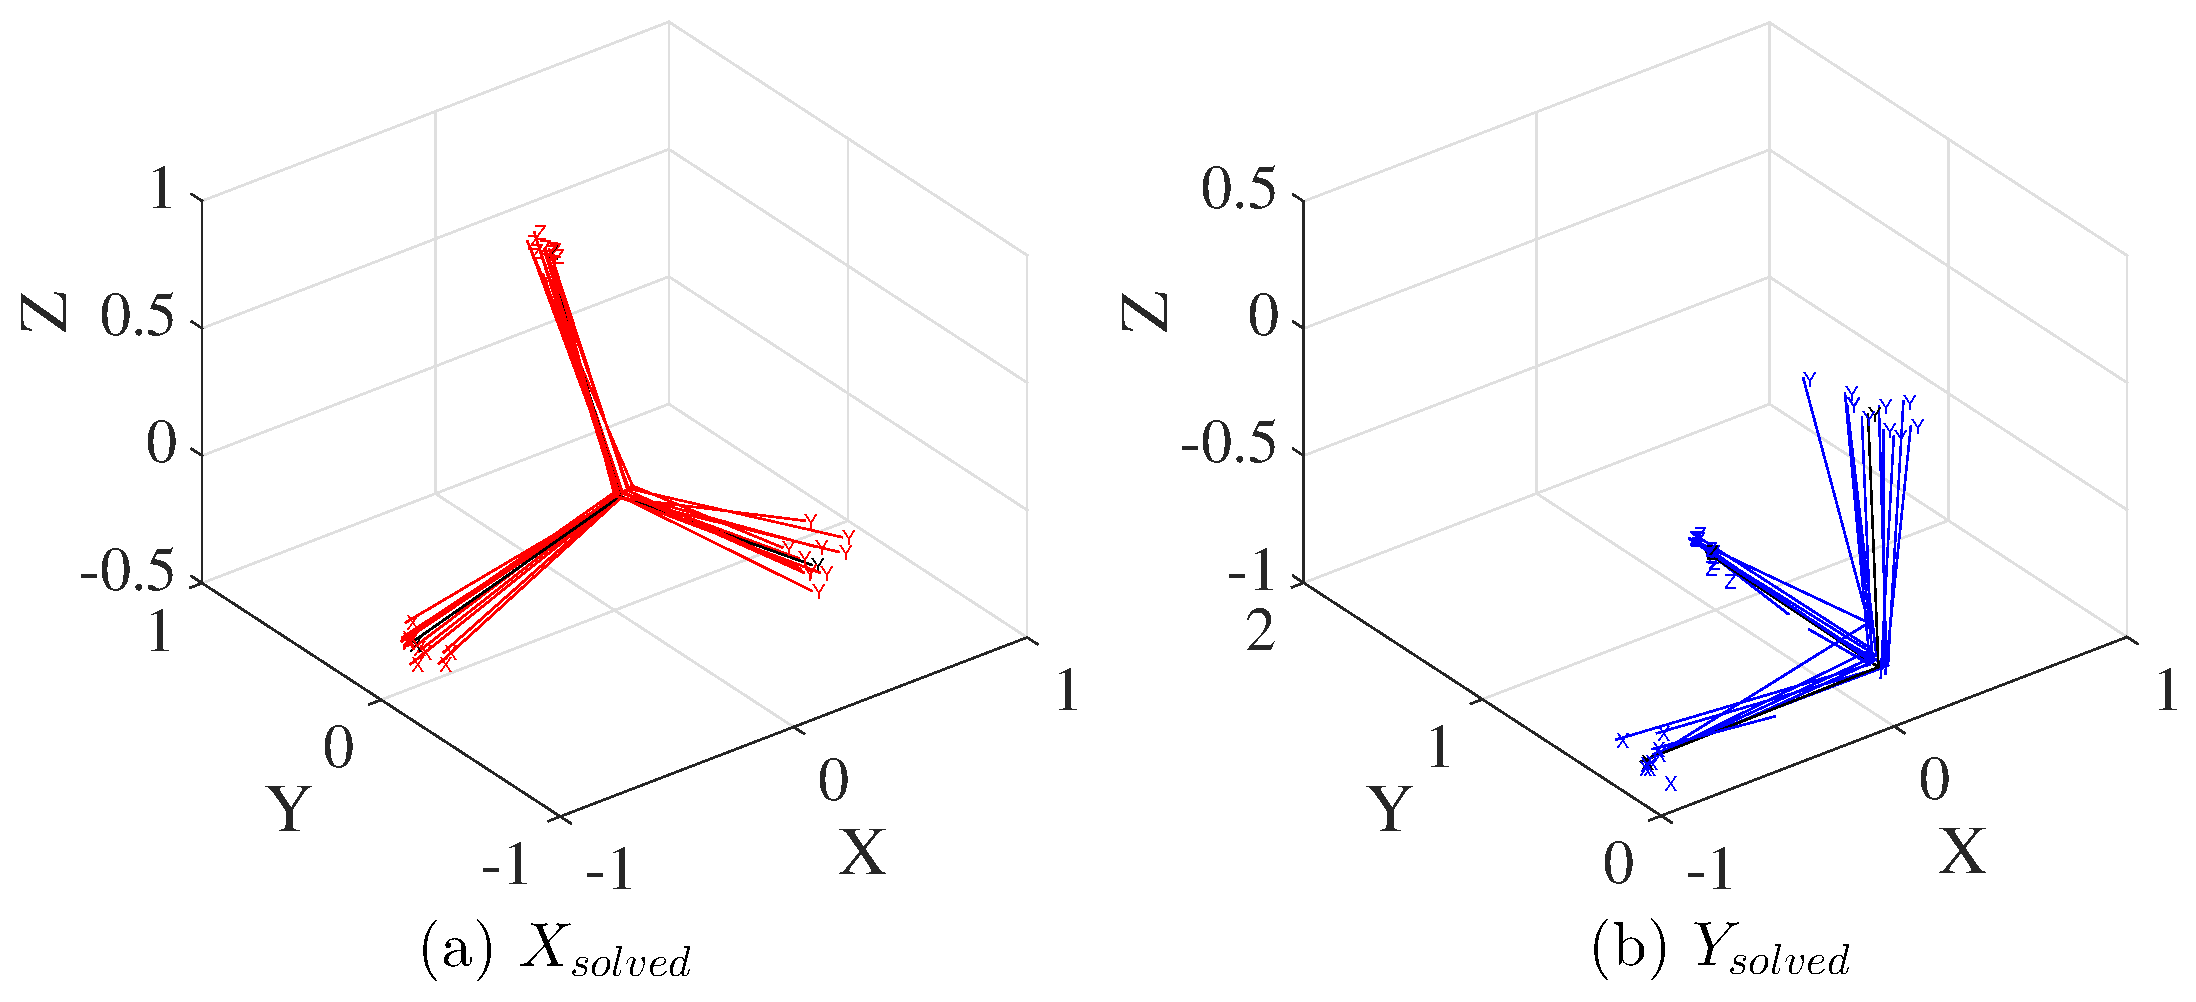
\includegraphics[width=3in]{fig4.eps}
\caption{
(a) The solved $X$ (in red) and the actual $X$ (in black) for 10 trials of simulation with noise covariance 0.05 and shift 2.(b) The solved $Y$ (in blue) and the actual $Y$ (in black) for 10 trials of simulation with noise covariance 0.05 and shift 2.
}
\label{fig4}
\end{figure}
\end{center}

There are multiple ways of generating the data streams $\{A_i\}$ and $\{B_{i}\}$. One way is to first generate $\{B_i\}$ and then map it to $\{A_i\}$ using $A = YBX^{-1}$. $\{B_i\}$ can be obtained by randomly sampling on the Lie algebra of $B$ from a zero mean multivariate Gaussian distribution, where the mean $\mu = {\bf 0} \in se(3)$ and covariance matrix $\Sigma \in \mathbb{R}^{6 \times 6}$ are as follows:

\begin{IEEEeqnarray}{l}
\delta_i \in \mathcal{N}({\bf 0};\Sigma) \subset \mathbb{R}^{6} \IEEEyessubnumber\label{equ28a}
\\*
B_i = \text{exp}(\hat{\delta_i}) \text{exp}(\mu) \IEEEyessubnumber\label{equ28b}
\end{IEEEeqnarray}

The data stream $\{A_i\}$ can be easily obtained as described above. After employing the proposed probabilistic method, 8 sets of sequences $(\theta_{A_{i}},\theta_{B_{i}^{k}})$ and $(d_{A_{i}},d_{B_{i}^{k}})$ where $ i = 1,\cdots, 100$ and $k = 1,\dots,8$ can be obtained respectively.

If the data streams $\{A_i\}$ were shifted by $m$ units compared to the data stream $\{B_i\}$, then the maximum of cross correlation can be used to recover the shift. Once done, we shift the data stream $\{A_i\}$ back to recover the correspondence, which can help find a correct solution satisfying the Euclidean-Group invariants using Eq.(\ref{equ22}). Therefore, only one pair of $(X_k, Y_k)$ can be picked to minimize the cost function. In Fig.~\ref{fig2}, because the shift between $\{A_i\}$ and $\{B_i\}$ were calculated accurately, the errors of translations and rotations increase remain similar as that of non-shift data streams.


To test the robustness of the proposed method, noises are exerted to $\{B_i\}$ by the data stream $B_i^{noise} = B_i \text{exp}(\mathbf{\widehat{x}}_{noise})$, where each element of the Lie Algebra $\mathbf{x}_{noise}$ is a Gaussian distribution as $N \sim (\mu_{noise},\sigma_{noise})$. In Fig.~\ref{fig3}, as $\sigma_{noise}$ increments from $0.01$ to $0.08$, the errors of $R_X$, $R_Y$, $t_X$, and $t_Y$ increase as shown in the box-and-whisker plot. There are several outliers outside the whiskers. The median value can be used as the final solved $X$ and $Y$. Fig.~\ref{fig4} show the solved ($X$,$Y$)s in red and blue with the actual ($X$,$Y$) in black in the coordinate frame when the noise covariance is 0.05 and shift is 2.

\begin{center}
\begin{figure}
\centering
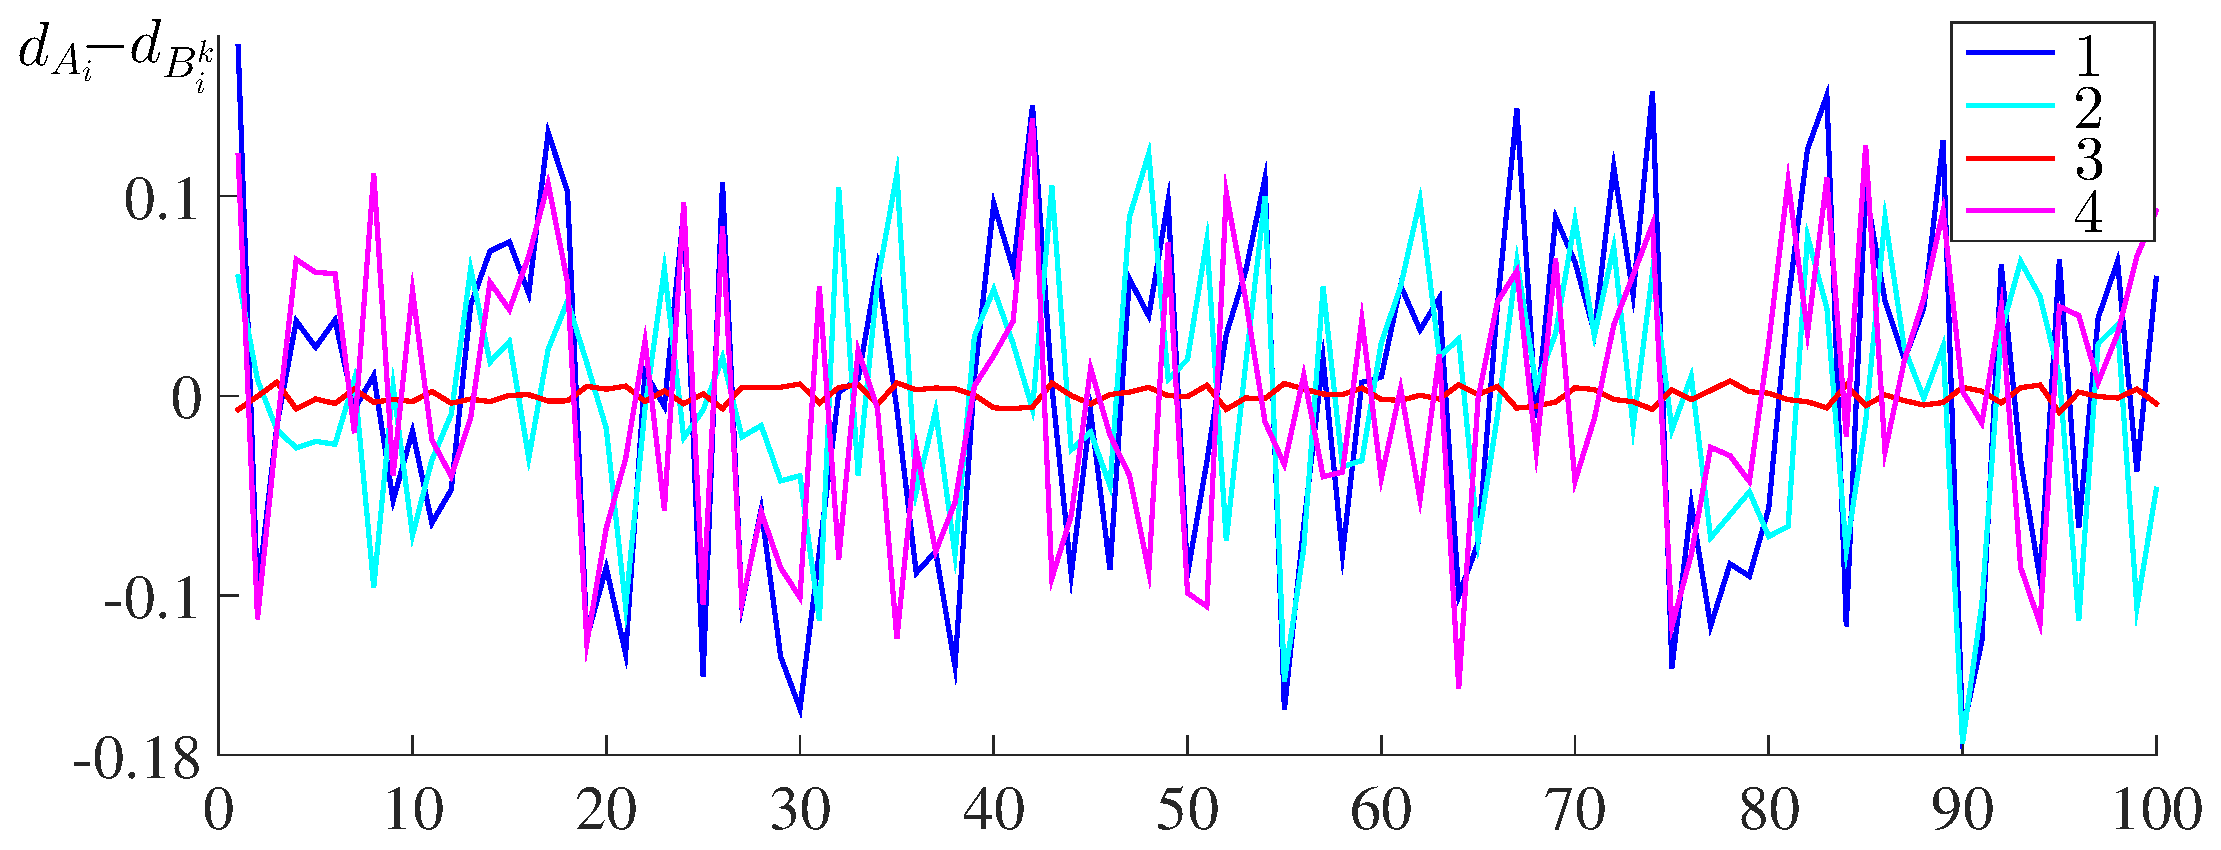
\includegraphics[width=3in]{fig5.eps}
\caption{
Error of orientation and position of $X$ and $Y$ versus shift amount when using Li and Shah method without regaining the correspondence.
}
\label{fig5}
\end{figure}
\end{center}

\begin{center}
\begin{figure}
\centering
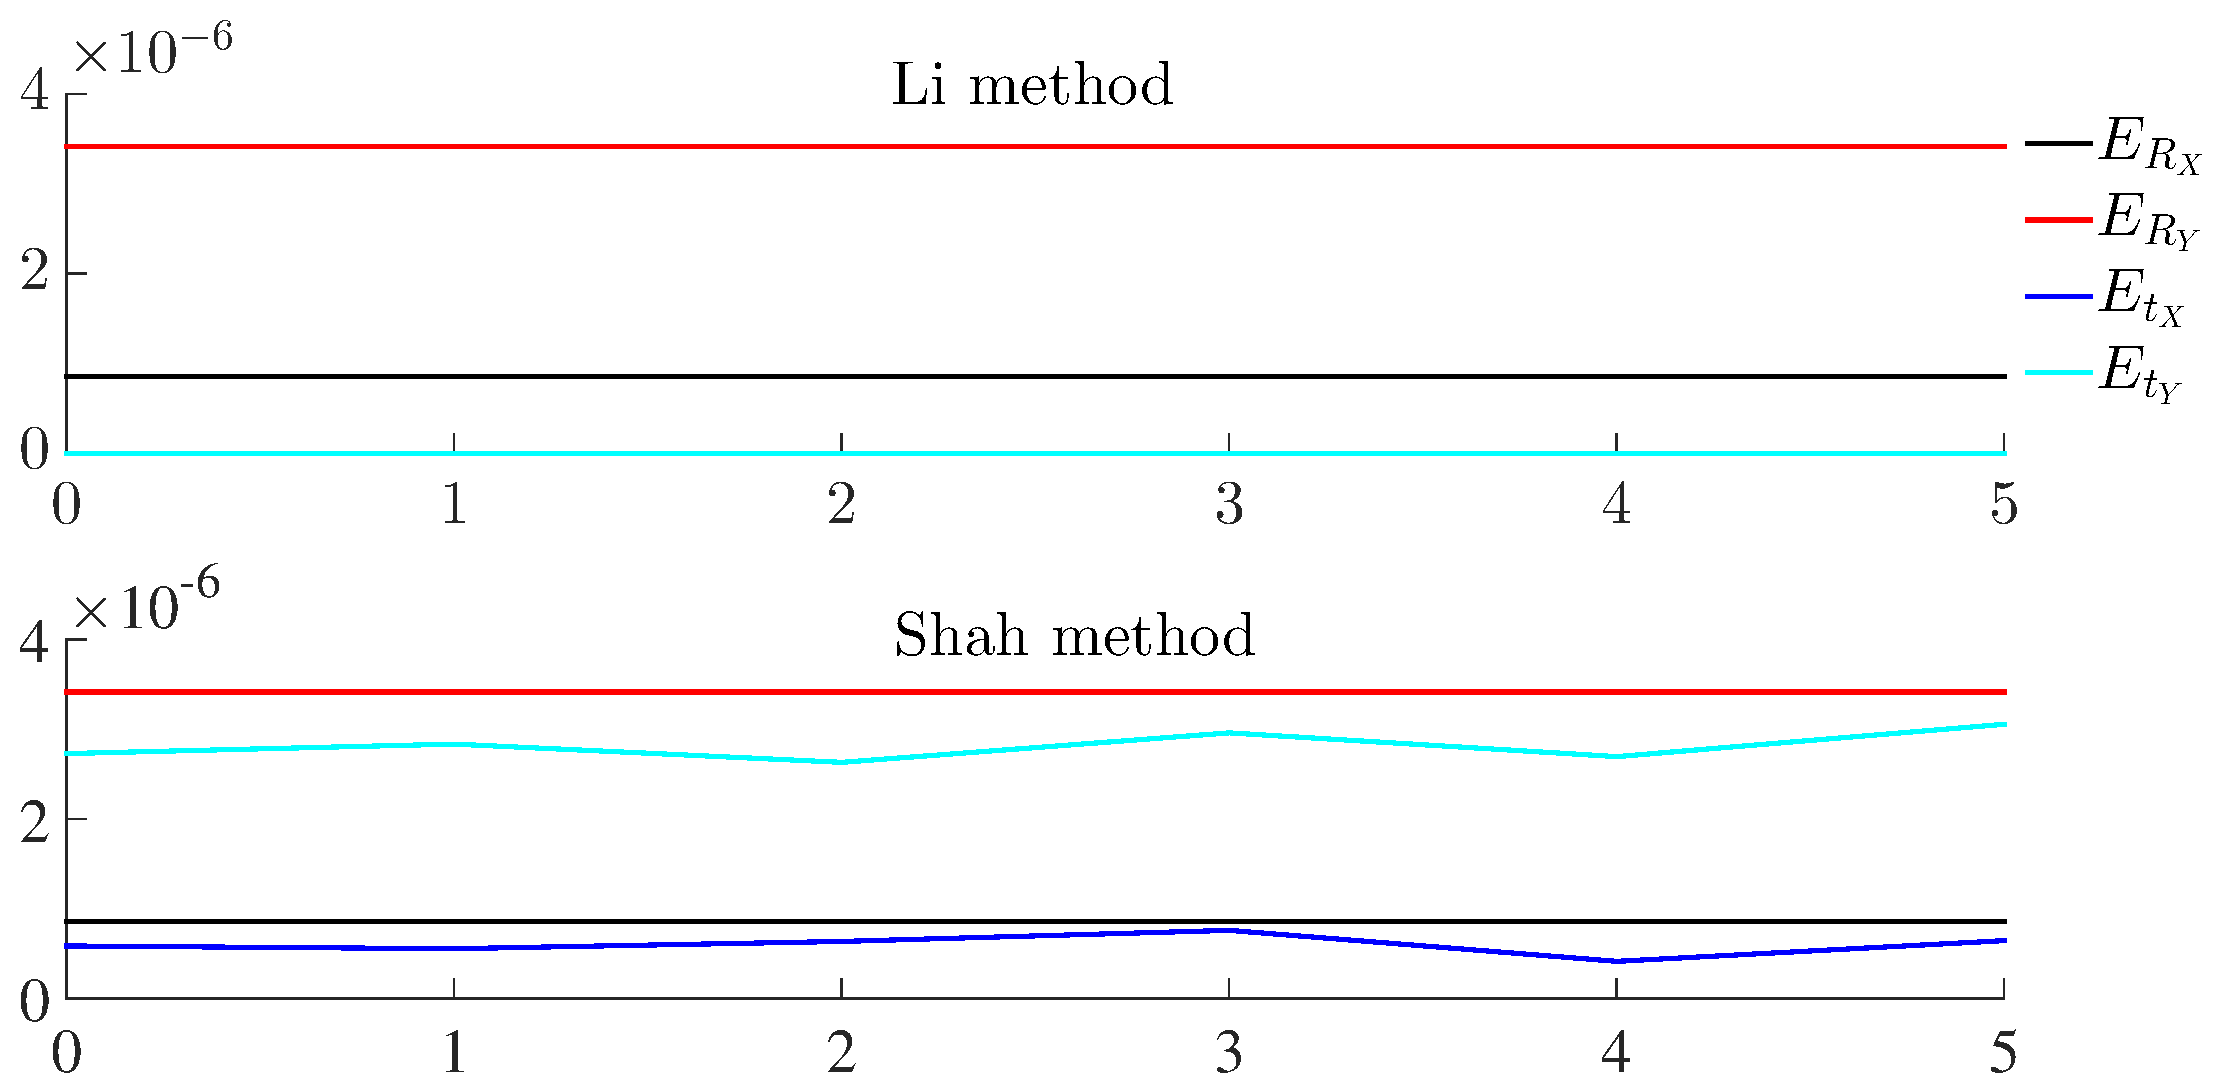
\includegraphics[width=3in]{fig6.eps}
\caption{
Error of orientation and position of $X$ and $Y$ versus shift amount when using Li and Shah method after regaining correspondence.
}
\label{fig6}
\end{figure}
\end{center}
The probabilistic method in this paper can regain the correspondence of the shifted data streams, which is useful for other sensor calibration methods. In $AX=YB$ problem, there have been many calibration methods that have been developed for solving $AX=YB$ problem. However, few of them considered the cases without correspondence. When data streams of ${A}$ and ${B}$ are shifted or asynchronous, the solution is unavailable. We shift the data sequence of ${A}$ by $n=0,1,2,3,4,5$ with respect to the data sequence of ${B}$. We combine the probabilistic method with other methods. In Li's method \cite{Li2010}, $X$ and $Y$ are solved for at the same time while Shah \cite{Shah2013} uses separable solutions to solve for $X$ and $Y$. In Fig.~\ref{fig5}, the correspondence between data streams are still unknown and the errors are obvious. After the data streams are synchronized using the probabilistic method in Fig.~\ref{fig6}, Li and Shah's methods work as well as that in non-shift situation.

\section{Conclusions}
\label{sect5}

In this paper, we developed a probabilistic approach to simultaneously obtain  $X$ and $Y$ in $AX=YB$ sensor calibration problem. Without a prior knowledge of the correspondence between $\{A_i\}$ and $\{B_j\}$, the proposed probabilistic method on Lie group is used to constrain the possible solutions of $X$ and $Y$ to eight pairs of candidates. Given shifted data streams of $\{A_{i+s}\}$ and $\{B_i\}$, using the correlation theorem with Euclidean group invariants,the correspondence is recovered to determine the correct solution among the eight candidates. In the numerical simulation, the method performs well with different sets of data samples.
%\section{Conclusion}
% conference papers do not normally have an appendix

\addtolength{\textheight}{-12cm}   % This command serves to balance the column lengths
                                  % on the last page of the document manually. It shortens
                                  % the textheight of the last page by a suitable amount.
                                  % This command does not take effect until the next page
                                  % so it should come on the page before the last. Make
                                  % sure that you do not shorten the textheight too much.

%%%%%%%%%%%%%%%%%%%%%%%%%%%%%%%%%%%%%%%%%%%%%%%%%%%%%%%%%%%%%%%%%%%%%%%%%%%%%%%%



%%%%%%%%%%%%%%%%%%%%%%%%%%%%%%%%%%%%%%%%%%%%%%%%%%%%%%%%%%%%%%%%%%%%%%%%%%%%%%%%



%%%%%%%%%%%%%%%%%%%%%%%%%%%%%%%%%%%%%%%%%%%%%%%%%%%%%%%%%%%%%%%%%%%%%%%%%%%%%%%%

\section*{ACKNOWLEDGMENT}



%%%%%%%%%%%%%%%%%%%%%%%%%%%%%%%%%%%%%%%%%%%%%%%%%%%%%%%%%%%%%%%%%%%%%%%%%%%%%%%%


\bibliographystyle{IEEEtran}
\bibliography{IEEEabrv,bibIEEEfull}
%\begin{thebibliography}{1}
%
%
%\end{thebibliography}

\end{document}
